\documentclass{article}

\usepackage{tikz}
\usepackage{graphicx}
\usetikzlibrary{arrows.meta}

% ---------- Colors ----------
\definecolor{navy}{RGB}{20,55,100}
\definecolor{steel}{RGB}{70,100,130}
\definecolor{gold}{RGB}{190,140,40}
\definecolor{goldpale}{RGB}{255,248,220}
\definecolor{green}{RGB}{45,140,85}
\definecolor{greenpale}{RGB}{230,248,238}
\definecolor{red}{RGB}{190,60,60}
\definecolor{redpale}{RGB}{255,235,235}
\definecolor{bluepale}{RGB}{235,242,250}

\begin{document}
	
	\begin{figure}[ht]
		\centering
		
		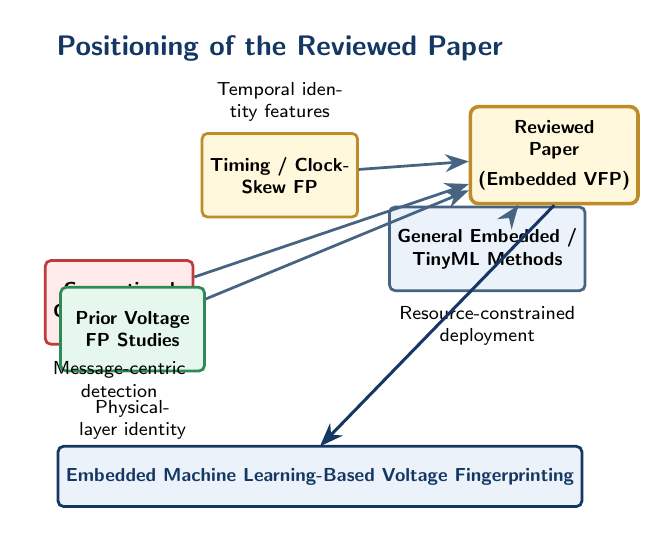
\begin{tikzpicture}[scale=0.85, transform shape]
			
			% ==================================================
			% TITLE
			% ==================================================
			
			\node[
			font=\sffamily\bfseries\large,
			text=navy,
			align=center
			] at (4.2,4.8)
			{Positioning of the Reviewed Paper};
			
			% ==================================================
			% COMPARISON NODES
			% ==================================================
			
			\node[
			rectangle,
			rounded corners=2pt,
			draw=red,
			fill=redpale,
			line width=1pt,
			minimum width=2.15cm,
			minimum height=1.25cm,
			align=center,
			font=\sffamily\bfseries\footnotesize
			] (a) at (1.8,1.0)
			{\textbf{Conventional}\\
				\textbf{CAN IDS/ADS}};
			
			\node[
			rectangle,
			rounded corners=2pt,
			draw=gold,
			fill=goldpale,
			line width=1pt,
			minimum width=2.15cm,
			minimum height=1.25cm,
			align=center,
			font=\sffamily\bfseries\footnotesize
			] (b) at (4.2,2.9)
			{\textbf{Timing / Clock-}\\
				\textbf{Skew FP}};
			
			\node[
			rectangle,
			rounded corners=2pt,
			draw=green,
			fill=greenpale,
			line width=1pt,
			minimum width=2.15cm,
			minimum height=1.25cm,
			align=center,
			font=\sffamily\bfseries\footnotesize
			] (c) at (2.0,0.6)
			{\textbf{Prior Voltage}\\
				\textbf{FP Studies}};
			
			\node[
			rectangle,
			rounded corners=2pt,
			draw=steel,
			fill=bluepale,
			line width=1pt,
			minimum width=2.15cm,
			minimum height=1.25cm,
			align=center,
			font=\sffamily\bfseries\footnotesize
			] (d) at (7.3,1.8)
			{\textbf{General Embedded /}\\
				\textbf{TinyML Methods}};
			
			% ==================================================
			% REVIEWED PAPER
			% ==================================================
			
			\node[
			rectangle,
			rounded corners=3pt,
			draw=gold,
			fill=goldpale,
			line width=1.3pt,
			minimum width=2.45cm,
			minimum height=1.45cm,
			align=center,
			font=\sffamily\bfseries\footnotesize
			] (e) at (8.3,3.2)
			{\textbf{Reviewed}\\
				\textbf{Paper}\\[1mm]
				\textbf{(Embedded VFP)}};
			
			% ==================================================
			% CONNECTIONS
			% ==================================================
			
			\draw[
			-{Stealth[length=3mm]},
			line width=1pt,
			draw=steel
			] (a) -- (e);
			
			\draw[
			-{Stealth[length=3mm]},
			line width=1pt,
			draw=steel
			] (b) -- (e);
			
			\draw[
			-{Stealth[length=3mm]},
			line width=1pt,
			draw=steel
			] (c) -- (e);
			
			\draw[
			-{Stealth[length=3mm]},
			line width=1pt,
			draw=steel
			] (d) -- (e);
			
			% ==================================================
			% LABELS
			% ==================================================
			
			\node[
			font=\sffamily\footnotesize,
			text width=2.5cm,
			align=center
			] at (1.8,-0.15)
			{Message-centric detection};
			
			\node[
			font=\sffamily\footnotesize,
			text width=2.5cm,
			align=center
			] at (4.2,4.0)
			{Temporal identity features};
			
			\node[
			font=\sffamily\footnotesize,
			text width=2.5cm,
			align=center
			] at (2.0,-0.75)
			{Physical-layer identity};
			
			\node[
			font=\sffamily\footnotesize,
			text width=2.8cm,
			align=center
			] at (7.3,0.65)
			{Resource-constrained deployment};
			
			% ==================================================
			% BOTTOM MESSAGE
			% ==================================================
			
			\node[
			rectangle,
			rounded corners=2pt,
			draw=navy,
			fill=bluepale,
			line width=1pt,
			minimum width=7cm,
			minimum height=0.9cm,
			align=center,
			font=\sffamily\bfseries\footnotesize,
			text=navy
			] at (4.8,-1.6)
			{Embedded Machine Learning-Based Voltage Fingerprinting};
			
			\draw[
			-{Stealth[length=3mm]},
			line width=1.1pt,
			draw=navy
			] (e.south) -- (4.8,-1.15);
			
		\end{tikzpicture}
		
		\caption{Comparative positioning of the reviewed paper relative to conventional IDS, timing fingerprinting, prior voltage fingerprinting studies, and general embedded TinyML methods.}
		
		\label{fig:positioning}
		
	\end{figure}
	
\end{document}